\documentclass[12pt,a4paper]{article}
\usepackage[utf8]{inputenc}
\usepackage[T1]{fontenc}
\usepackage{amsmath,amssymb}
\usepackage{graphicx}
\usepackage{booktabs}
\usepackage[margin=2.5cm]{geometry}
\usepackage{caption}
\usepackage{subcaption}
\usepackage{float}
\usepackage{hyperref}
\usepackage{array}
\usepackage{multirow}

\graphicspath{{figures/}}

\title{\textbf{Evolutionary Analysis of the Iterated Symmetric Centipede Game}\\[0.5em]
\large with All-$M/2$, All-$1$, and Grim Strategies}
\author{}
\date{}

\begin{document}

\maketitle
\tableofcontents
\newpage

% ============================================================
\section{Introduction}
% ============================================================

This report presents the numerical results of an evolutionary game-theoretic
analysis of the \textbf{Iterated Symmetric Centipede (ISC)} game, based on the
work of Lazaridis and Kehagias~\cite{LK2026}. The analysis studies the
co-evolutionary dynamics of three strategies --- All-$M/2$, All-$1$, and Grim
--- under both continuous Replicator Dynamics and discrete Markov Chain
Dynamics.

The key modification with respect to the original paper is the replacement of
the \textbf{All-$M$} strategy with \textbf{All-$M/2$}, which cooperates at the
midpoint level $\rho_{M/2}$ rather than the maximum $\rho_M$. This single
change alters the payoff matrix, the set of absorbing states, and the
equilibrium structure in important ways that are documented throughout this
report.

The MATLAB implementation delivers:
\begin{itemize}
  \item functions \texttt{xRepDyn}, \texttt{PhasePlot}, \texttt{PStateTransitionGraph}, \texttt{sMarkDyn};
  \item scripts \texttt{xRep001} and \texttt{xMark001} that reproduce
        Figures~2--5 of~\cite{LK2026} and provide extended parameter
        sensitivity analysis.
\end{itemize}

% ============================================================
\section{The ISC Game Model}
% ============================================================

\subsection{The One-Shot Symmetric Centipede (OSC)}

The OSC is a two-player extensive-form game with $M$ stages. At each stage
$i$, the active player may \emph{terminate} (take action $\rho_i$, ending the
game) or \emph{pass} the move to the opponent. The first player to terminate
receives a share $p \in (1/2, 1]$ of the joint payoff, while the passive player
receives the complementary share $1-p$.

The resulting payoff matrix $A$ (to the row player) is:
\[
  A(i,j) = \begin{cases}
    i                  & \text{if } i = j \\
    (2i+1)\,p          & \text{if } i < j \\
    (2j+1)\,(1-p)      & \text{if } i > j
  \end{cases}
\]

\subsection{The Iterated Symmetric Centipede (ISC)}

The ISC consists of $T$ repeated plays of the OSC. In each round the
first-moving player is selected uniformly at random, so each player moves first
in half the rounds on average.

\subsection{Strategies}

Three ISC strategies are studied (default parameters: $M=4$, $k = M/2 = 2$):

\begin{center}
\begin{tabular}{cllp{7cm}}
\toprule
Index & Symbol & Name & Description \\
\midrule
1 & $\sigma_{\text{All-}M/2}$ & All-$M/2$ &
    Always play $\rho_{M/2}$: cooperates at the mid-level. \\
2 & $\sigma_{\text{All-}1}$   & All-$1$ &
    Always play $\rho_1$: always defects immediately. \\
3 & $\sigma_G$                & Grim &
    Play $\rho_M$ in round 1; if the opponent ever plays $\rho_m$ with
    $m < M$, switch permanently to $\rho_1$. \\
\bottomrule
\end{tabular}
\end{center}

\medskip
\noindent\textbf{Grim trigger rule.} The trigger condition is $m < M$:
\begin{itemize}
  \item Grim \emph{triggers} against All-$M/2$ (plays $\rho_{M/2}$, and $M/2 < M$).
  \item Grim \emph{triggers} against All-$1$ (plays $\rho_1$, and $1 < M$).
  \item Grim does \emph{not} trigger against another Grim (plays $\rho_M$, and $M \not< M$).
\end{itemize}
Consequently, two Grim players cooperate at the highest level every round,
yielding the self-play payoff $C(3,3) = T \cdot M$.

% ============================================================
\section{The ISC Payoff Matrix \texorpdfstring{$C$}{C}}
% ============================================================

\subsection{Symbolic Form}

The entry $C(i,j)$ is the payoff to strategy $i$ when facing strategy $j$
over $T$ rounds of the OSC. The symbolic matrix is:

\[
C = \begin{bmatrix}
\dfrac{M}{2}\,T & 3(1-p)\,T & (M+1)p + (T-1)\,3(1-p) \\[10pt]
3p\,T & T & 3p + (T-1) \\[10pt]
(M+1)(1-p) + (T-1)\,3p & 3(1-p) + (T-1) & T\,M
\end{bmatrix}
\]

\begin{figure}[H]
  \centering
  \includegraphics[width=0.85\textwidth]{payoff_matrix_symbolic}
  \caption{Symbolic ISC payoff matrix $C$ displayed by \texttt{xPrintC.m}.}
  \label{fig:C_symbolic}
\end{figure}

\subsection{Entry Derivation}

\begin{table}[H]
\centering
\caption{Derivation of each $C(i,j)$ entry.}
\label{tab:C_derivation}
\small
\begin{tabular}{clccll}
\toprule
Cell & Matchup & Round 1 & Trigger? & Rounds $2\ldots T$ & Formula \\
\midrule
$C(1,1)$ & All-$M/2$ vs All-$M/2$ & $A(k,k)$ & No  & $A(k,k)$   & $T\cdot(M/2)$ \\
$C(1,2)$ & All-$M/2$ vs All-$1$   & $A(k,1)$ & No  & $A(k,1)$   & $3(1-p)\,T$ \\
$C(1,3)$ & All-$M/2$ vs Grim      & $A(k,M)$ & Yes & $A(k,1)$   & $(M+1)p+(T-1)\cdot3(1-p)$ \\
$C(2,1)$ & All-$1$ vs All-$M/2$   & $A(1,k)$ & No  & $A(1,k)$   & $3p\,T$ \\
$C(2,2)$ & All-$1$ vs All-$1$     & $A(1,1)$ & No  & $A(1,1)$   & $T$ \\
$C(2,3)$ & All-$1$ vs Grim        & $A(1,k)$ & Yes & $A(1,1)$   & $3p+(T-1)$ \\
$C(3,1)$ & Grim vs All-$M/2$      & $A(M,k)$ & Yes & $A(1,k)$   & $(M+1)(1-p)+(T-1)\cdot3p$ \\
$C(3,2)$ & Grim vs All-$1$        & $A(M,1)$ & Yes & $A(1,1)$   & $3(1-p)+(T-1)$ \\
$C(3,3)$ & Grim vs Grim           & $A(M,M)$ & No  & $A(M,M)$   & $T\cdot M$ \\
\bottomrule
\end{tabular}
\end{table}

\subsection{Numerical Values ($M=4$, $T=10$)}

\begin{table}[H]
\centering
\caption{Numerical payoff matrix $C$ for $p=3/4$, $M=4$, $T=10$.}
\label{tab:C_p075}
\begin{tabular}{lccc}
\toprule
           & vs All-$M/2$ & vs All-$1$ & vs Grim \\
\midrule
All-$M/2$  & 20    & 7.5   & 10.5   \\
All-$1$    & 22.5  & 10    & 11.25  \\
Grim       & 21.5  & 9.75  & 40     \\
\bottomrule
\end{tabular}
\end{table}

\begin{table}[H]
\centering
\caption{Numerical payoff matrix $C$ for $p=3/5$, $M=4$, $T=10$.}
\label{tab:C_p060}
\begin{tabular}{lccc}
\toprule
           & vs All-$M/2$ & vs All-$1$ & vs Grim \\
\midrule
All-$M/2$  & 20    & 12    & 13.8   \\
All-$1$    & 18    & 10    & 10.8   \\
Grim       & 18.2  & 10.2  & 40     \\
\bottomrule
\end{tabular}
\end{table}

\noindent\textbf{Why Grim dominates.} The diagonal self-play payoffs are:
All-$M/2$: $T \cdot (M/2) = 20$; \quad All-$1$: $T = 10$; \quad
Grim: $T \cdot M = 40$.
Grim earns twice the payoff of All-$M/2$ in a homogeneous population because
it cooperates at $\rho_M$ (without triggering against other Grims).

% ============================================================
\section{Replicator Dynamics}
% ============================================================

\subsection{Model}

Let $x = (x_1, x_2, x_3)$ denote the population frequencies of All-$M/2$,
All-$1$, and Grim respectively, with $x_1+x_2+x_3=1$ and $x_i \geq 0$. The
replicator equation is:
\[
  \dot{x}_m = x_m \left[ (Cx)_m - x^\top C x \right], \quad m = 1,2,3.
\]

\subsection{Phase Portraits (Figures 2--3 of \cite{LK2026})}

\begin{figure}[H]
  \centering
  \begin{subfigure}[b]{0.48\textwidth}
    
\includegraphics[width=\textwidth]{rep_phase_p075}
    \caption{$p = 3/4$}
    \label{fig:phase_p075}
  \end{subfigure}
  \hfill
  \begin{subfigure}[b]{0.48\textwidth}
    
\includegraphics[width=\textwidth]{rep_phase_p060}
    \caption{$p = 3/5$}
    \label{fig:phase_p060}
  \end{subfigure}
  \caption{Phase portraits of the replicator dynamics ($M=4$, $T=10$).
           Axes: $x_1$ = All-$M/2$ frequency, $x_2$ = All-$1$ frequency.
           The third coordinate $x_3 = 1-x_1-x_2$ is implicit.}
  \label{fig:phase_both}
\end{figure}

\subsection{Time Series}

\begin{figure}[H]
  \centering
  \begin{subfigure}[b]{0.48\textwidth}
    
\includegraphics[width=\textwidth]{rep_timeseries_p075}
    \caption{$p = 3/4$}
  \end{subfigure}
  \hfill
  \begin{subfigure}[b]{0.48\textwidth}
    
\includegraphics[width=\textwidth]{rep_timeseries_p060}
    \caption{$p = 3/5$}
  \end{subfigure}
  \caption{Replicator dynamics time series ($M=4$, $T=10$, random initial condition).}
  \label{fig:rep_timeseries}
\end{figure}

\subsection{Rest Points and Stability}

The rest points of the replicator dynamics satisfy $(Cx)_m = x^\top Cx$ for
all $m$ with $x_m > 0$. The three pure-strategy vertices are always rest
points; additional edge and interior equilibria may exist depending on parameters.

Key analytical results from~\cite{LK2026} (adapted to All-$M/2$):
\begin{itemize}
  \item The set $\{(x_1, 0, 1-x_1) : x_1 \in [0,1]\}$ (the All-$M/2$--Grim
        edge, with no defectors) is always a stable equilibrium set; all
        trajectories converge to it.
  \item The pure-defector vertex $(0,1,0)$ has Jacobian eigenvalues
        $[-T,\;-(3p-2),\;-T(3p-2)]$ at All-$1$:
        \begin{itemize}
          \item $p > 2/3$ (e.g.\ $p=3/4$): all eigenvalues negative $\Rightarrow$
                $(0,1,0)$ is \textbf{asymptotically stable}.
          \item $p < 2/3$ (e.g.\ $p=3/5$): second and third eigenvalues
                positive $\Rightarrow$ $(0,1,0)$ is \textbf{unstable}.
        \end{itemize}
\end{itemize}

The numerical rest point analysis (computed by \texttt{RestPoints.m} for all
parameter combinations) is saved in \texttt{figures/restpoints.txt}.

\subsection{Parameter Sensitivity}

\begin{figure}[H]
  \centering
  
\includegraphics[width=\textwidth]{rep_overlay_vary_p}
  \caption{Replicator dynamics: effect of varying $p \in \{3/5,\,2/3,\,3/4,\,9/10\}$
           ($M=4$, $T=10$). Each subplot shows one strategy's frequency over time.}
  \label{fig:rep_vary_p}
\end{figure}

\begin{figure}[H]
  \centering
  
\includegraphics[width=\textwidth]{rep_overlay_vary_M}
  \caption{Replicator dynamics: effect of varying $M \in \{2,4,6,8\}$
           ($p=3/4$, $T=10$).}
  \label{fig:rep_vary_M}
\end{figure}

\begin{figure}[H]
  \centering
  
\includegraphics[width=\textwidth]{rep_overlay_vary_T}
  \caption{Replicator dynamics: effect of varying $T \in \{2,5,10,20\}$
           ($p=3/4$, $M=4$).}
  \label{fig:rep_vary_T}
\end{figure}

\subsection{Initial Condition Sensitivity}

\begin{figure}[H]
  \centering
  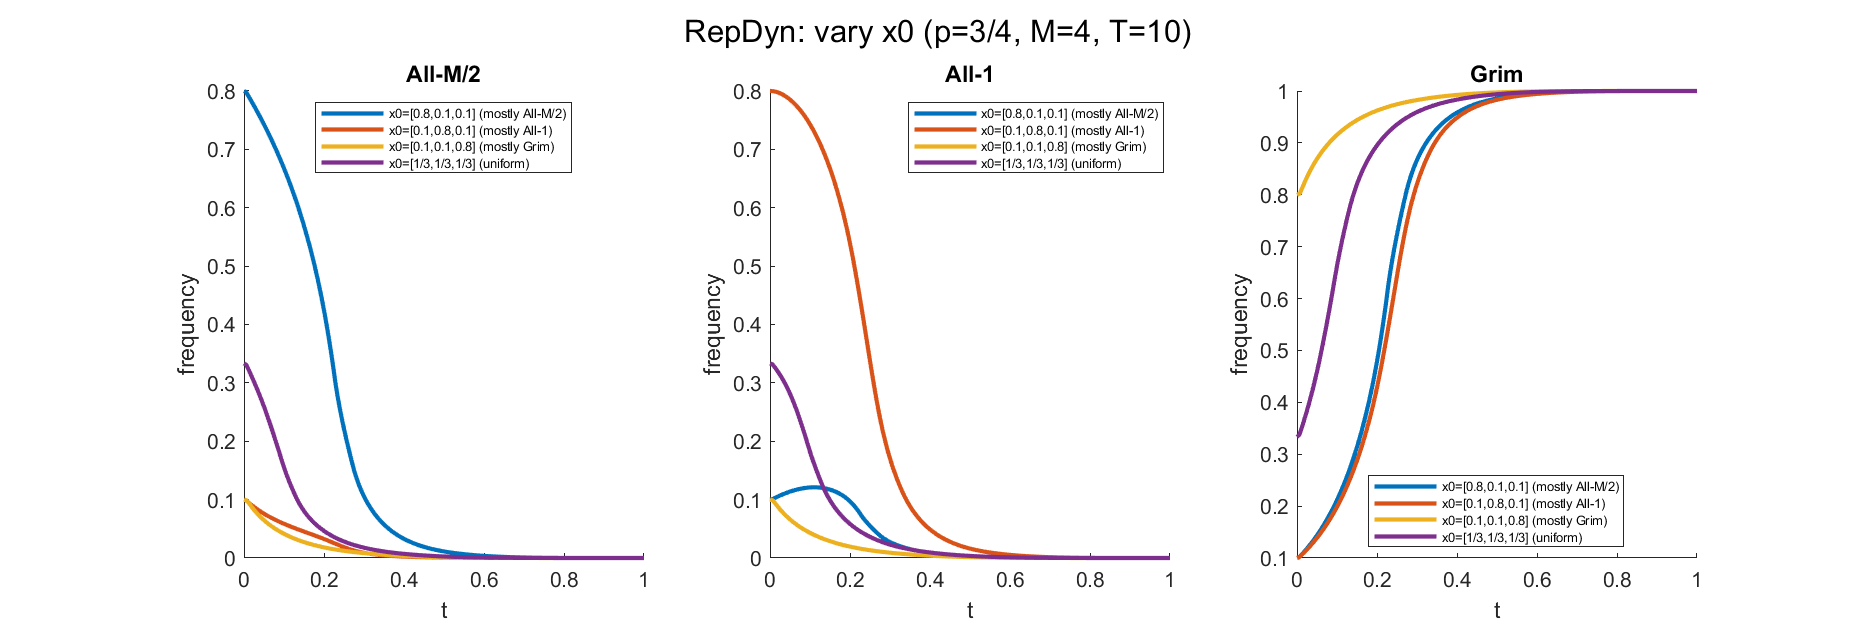
\includegraphics[width=\textwidth]{rep_overlay_vary_x0_p075}
  \caption{Replicator dynamics: effect of varying initial condition $x_0$
           ($p=3/4$, $M=4$, $T=10$).}
  \label{fig:rep_x0_p075}
\end{figure}

\begin{figure}[H]
  \centering
  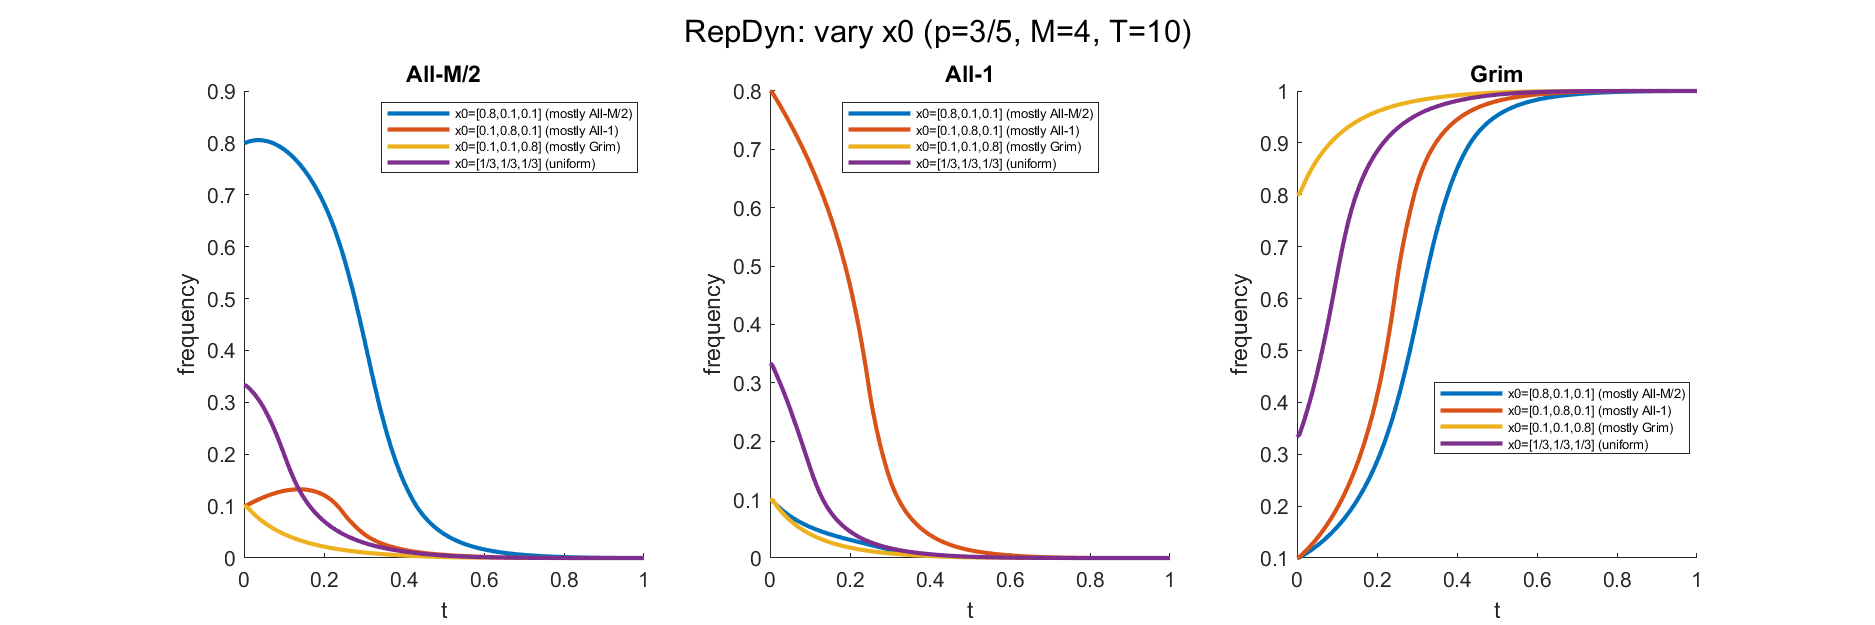
\includegraphics[width=\textwidth]{rep_overlay_vary_x0_p060}
  \caption{Replicator dynamics: effect of varying initial condition $x_0$
           ($p=3/5$, $M=4$, $T=10$).}
  \label{fig:rep_x0_p060}
\end{figure}

% ============================================================
\section{Markov Chain Dynamics}
% ============================================================

\subsection{Model}

The population state is $s = (s_1, s_2, s_3)$ with $s_1+s_2+s_3 = N$ and
$s_i \geq 0$ integers. There are $(N+1)(N+2)/2$ possible states. The
per-player payoff of strategy $m$ in state $s$ is:
\[
  q_m(s) = (s_m - 1)\,C(m,m) + \sum_{n \neq m} s_n\,C(m,n).
\]

Under the \textbf{Pairwise Proportional Imitation (PPI)} revision protocol, a
randomly selected All-$m_1$ player switches to All-$m_2$ with probability:
\[
  \varrho_{m_1 m_2}(s) =
  \frac{x_{m_2}\,[q_{m_2}(s) - q_{m_1}(s)]_+}
       {\sum_m x_m\,[q_m(s) - q_{m_1}(s)]_+}.
\]
The full transition matrix $P$ is built by \texttt{PStateTransitionGraph}.

\subsection{Absorbing States}

\noindent\textbf{Original paper (All-$M$):} The entire $s_2=0$ face is
absorbing because All-$M$ and Grim earn the same payoff $T \cdot M$ against
each other.

\noindent\textbf{This project (All-$M/2$):} $C(1,1) = T \cdot (M/2) = 20
\neq 40 = C(3,3)$, so Grim earns strictly more than All-$M/2$ on the $s_2=0$
face. All-$M/2$ players switch to Grim. The \textbf{only absorbing states} are
the three pure vertices:
$(N,0,0)$, $(0,N,0)$, $(0,0,N)$.

\subsection{State Transition Graphs (Figures 4--5 of \cite{LK2026})}

\begin{figure}[H]
  \centering
  \begin{subfigure}[b]{0.48\textwidth}
    
\includegraphics[width=\textwidth]{mark_stategraph_p075}
    \caption{$p = 3/4$}
    \label{fig:stategraph_p075}
  \end{subfigure}
  \hfill
  \begin{subfigure}[b]{0.48\textwidth}
    
\includegraphics[width=\textwidth]{mark_stategraph_p060}
    \caption{$p = 3/5$}
    \label{fig:stategraph_p060}
  \end{subfigure}
  \caption{Markov state transition graphs ($M=4$, $T=10$, $N=10$).
           Blue dots: absorbing (pure) states. Red dots: transient states.
           Arrow thickness indicates transition probability.}
  \label{fig:stategraph_both}
\end{figure}

\subsection{Time Series}

\begin{figure}[H]
  \centering
  \begin{subfigure}[b]{0.48\textwidth}
    
\includegraphics[width=\textwidth]{mark_timeseries_p075}
    \caption{$p = 3/4$}
  \end{subfigure}
  \hfill
  \begin{subfigure}[b]{0.48\textwidth}
    
\includegraphics[width=\textwidth]{mark_timeseries_p060}
    \caption{$p = 3/5$}
  \end{subfigure}
  \caption{Markov dynamics time series ($M=4$, $T=10$, $N=10$, $T_m=100$,
           $s_0=[3,4,3]$).}
  \label{fig:mark_timeseries}
\end{figure}

\subsection{Parameter Sensitivity}

\begin{figure}[H]
  \centering
  
\includegraphics[width=\textwidth]{mark_overlay_vary_p}
  \caption{Markov dynamics: effect of varying $p \in \{3/5,\,2/3,\,3/4,\,9/10\}$
           ($M=4$, $T=10$, $N=10$).}
  \label{fig:mark_vary_p}
\end{figure}

\begin{figure}[H]
  \centering
  
\includegraphics[width=\textwidth]{mark_overlay_vary_M}
  \caption{Markov dynamics: effect of varying $M \in \{2,4,6,8\}$
           ($p=3/4$, $T=10$, $N=10$).}
  \label{fig:mark_vary_M}
\end{figure}

\begin{figure}[H]
  \centering
  
\includegraphics[width=\textwidth]{mark_overlay_vary_T}
  \caption{Markov dynamics: effect of varying $T \in \{2,5,10,20\}$
           ($p=3/4$, $M=4$, $N=10$).}
  \label{fig:mark_vary_T}
\end{figure}

\begin{figure}[H]
  \centering
  
\includegraphics[width=\textwidth]{mark_overlay_vary_N}
  \caption{Markov dynamics: effect of varying $N \in \{5,10,15,20\}$
           ($p=3/4$, $M=4$, $T=10$).}
  \label{fig:mark_vary_N}
\end{figure}

\subsection{Initial State Sensitivity}

\begin{figure}[H]
  \centering
  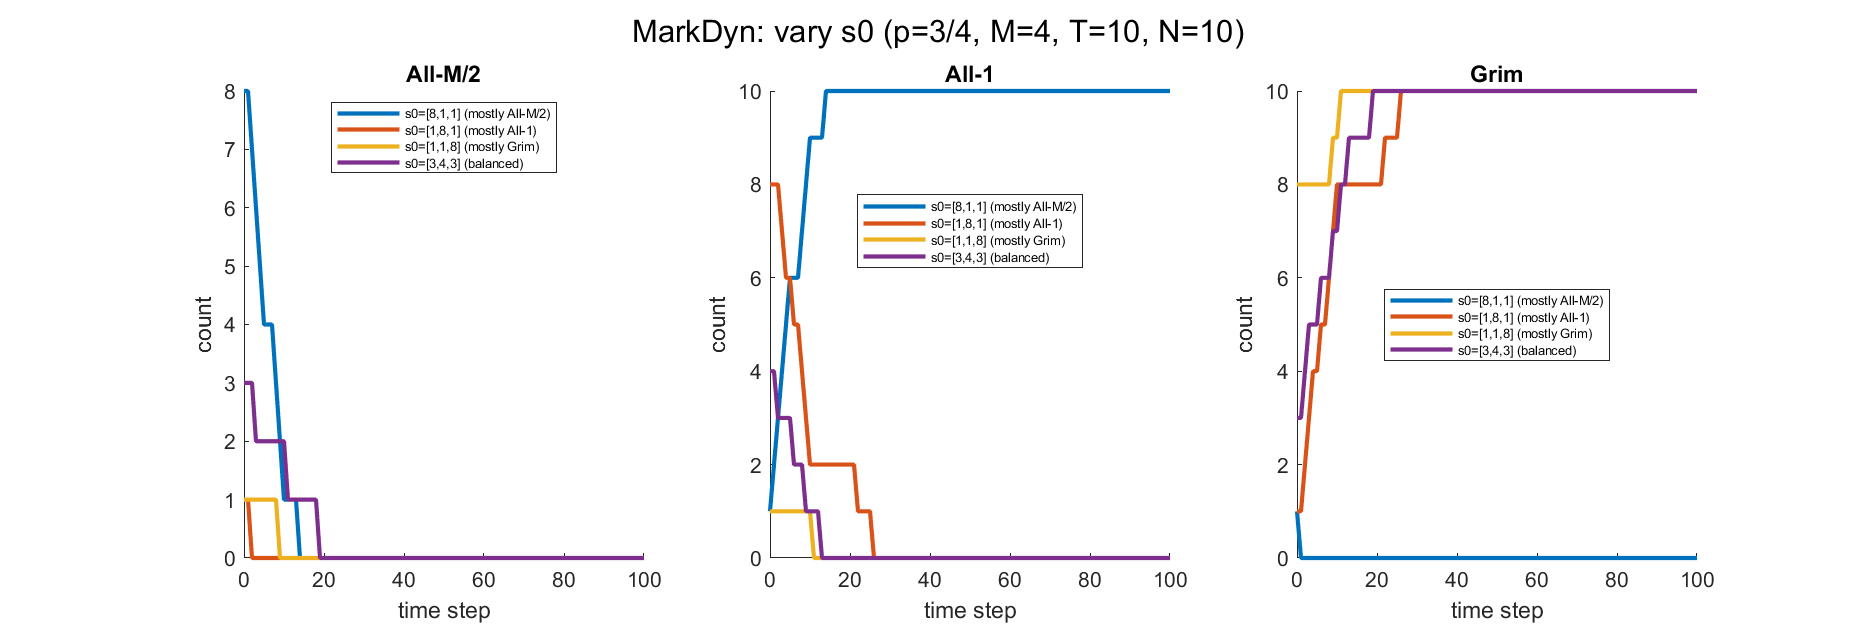
\includegraphics[width=\textwidth]{mark_overlay_vary_s0_p075}
  \caption{Markov dynamics: effect of varying initial state $s_0$
           ($p=3/4$, $M=4$, $T=10$, $N=10$).}
  \label{fig:mark_s0_p075}
\end{figure}

\begin{figure}[H]
  \centering
  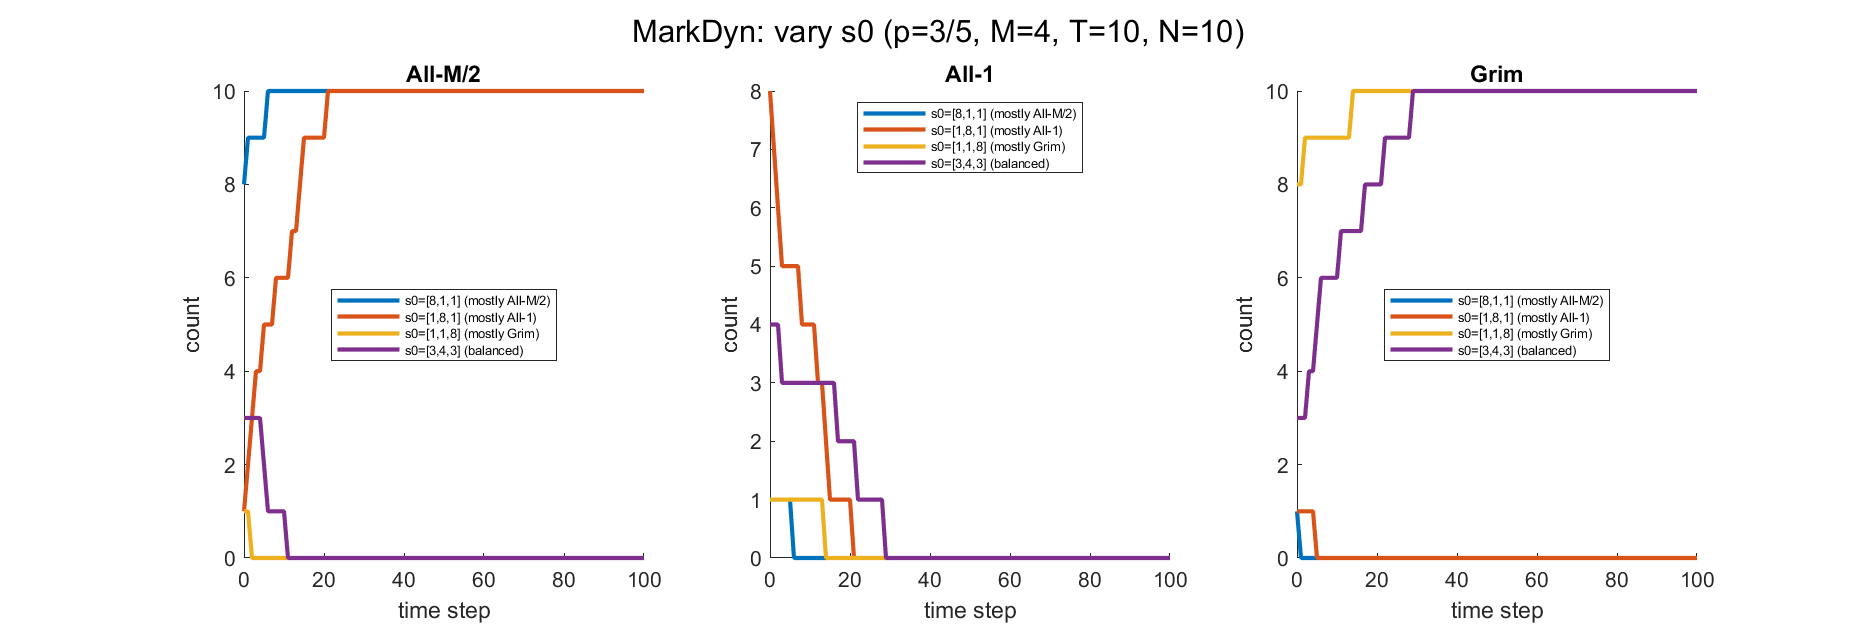
\includegraphics[width=\textwidth]{mark_overlay_vary_s0_p060}
  \caption{Markov dynamics: effect of varying initial state $s_0$
           ($p=3/5$, $M=4$, $T=10$, $N=10$).}
  \label{fig:mark_s0_p060}
\end{figure}

% ============================================================
\section{Discussion}
% ============================================================

\subsection{Effect of the All-\texorpdfstring{$M/2$}{M/2} Modification}

Table~\ref{tab:differences} summarises the key differences between the
original paper (which uses All-$M$) and this project (which uses All-$M/2$).

\begin{table}[H]
\centering
\caption{Comparison: original paper (All-$M$) vs.\ this project (All-$M/2$).}
\label{tab:differences}
\small
\begin{tabular}{lll}
\toprule
Aspect & Original (All-$M$) & This project (All-$M/2$) \\
\midrule
Cooperator strategy       & Always play $\rho_M$       & Always play $\rho_{M/2}$ \\
$C(1,1)$                  & $T \cdot M = 40$           & $T \cdot (M/2) = 20$ \\
$C(3,3)$                  & $T \cdot M = 40$           & $T \cdot M = 40$ (unchanged) \\
Grim trigger vs cooperator & Never ($M \not< M$)        & Always ($M/2 < M$) \\
$s_2{=}0$ face absorbing? & Yes (entire face)          & No (only pure vertices) \\
Absorbing states          & $(0,N,0)$ + $s_2{=}0$ face & $(N,0,0)$, $(0,N,0)$, $(0,0,N)$ \\
\bottomrule
\end{tabular}
\end{table}

\subsection{The \texorpdfstring{$p = 2/3$}{p = 2/3} Threshold}

A critical threshold emerges at $p = 2/3$:
\begin{itemize}
  \item $p > 2/3$ (e.g.\ $p = 3/4$): the pure-defector state $(0,1,0)$ is
        asymptotically stable. Both Grim and All-$1$ can be long-run outcomes.
  \item $p < 2/3$ (e.g.\ $p = 3/5$): $(0,1,0)$ is unstable. All-$1$ is
        driven out; the population converges to the All-$M/2$--Grim edge.
\end{itemize}
This threshold is visible in the phase portraits (Figure~\ref{fig:phase_both})
and confirmed by the Markov dynamics (Figure~\ref{fig:mark_vary_p}).

\subsection{Grim Dominance}

Grim is the uniquely dominant strategy in self-play ($C(3,3) = 40$, which is
twice $C(1,1) = 20$ and four times $C(2,2) = 10$). In the Markov dynamics this
is reflected by the strong drift toward the pure-Grim absorbing state $(0,0,N)$,
regardless of the initial condition, especially when $p < 2/3$.

% ============================================================
\section{Conclusion}
% ============================================================

This project has reproduced and extended the numerical results of
Lazaridis--Kehagias~\cite{LK2026} for the ISC game with strategies All-$M/2$,
All-$1$, and Grim. The main findings are:

\begin{enumerate}
  \item The payoff matrix $C$ is analytically derived and numerically verified
        for both $p = 3/4$ and $p = 3/5$.
  \item Replicator dynamics phase portraits (Figures~2--3 of~\cite{LK2026})
        confirm the $p = 2/3$ stability threshold for the All-$1$ equilibrium.
  \item Markov state transition graphs (Figures~4--5 of~\cite{LK2026}) confirm
        that, because All-$M/2$ earns less than Grim in self-play, the $s_2=0$
        face is no longer absorbing: only the three pure states are.
  \item Extended parameter sensitivity analysis shows consistent effects:
        higher $p$ promotes All-$1$ stability; higher $M$ and $T$ amplify
        Grim's payoff advantage; initial conditions affect speed of convergence
        but not the qualitative long-run outcome.
\end{enumerate}

% ============================================================
\begin{thebibliography}{9}
\bibitem{LK2026}
  I.~Lazaridis and A.~Kehagias,
  \textit{Iterated Symmetric Centipede: Learning and Evolutionary Games},
  March 2026.
\end{thebibliography}

\end{document}
